

\documentclass[conference]{IEEEtran}
%\usepackage {makecell}
\usepackage {url}
\usepackage {graphicx}
%\usepackage {caption}
\usepackage {algorithm}
\usepackage {algorithmic}
%\usepackage {algpseudocode}
\usepackage{amsmath}
\usepackage{tabu}
\usepackage[numbers,sort&compress]{natbib}
\usepackage{bbding}
% correct bad hyphenation here
\hyphenation{op-tical net-works semi-conduc-tor}

\begin{document}
% paper title
\title{Joint Energy-Aware and Buffer-Assisted Relay Selection Method for Relay-Aided D2D Communications}

% author names and affiliations
% use a multiple column layout for up to three different
% affiliations
\author{\IEEEauthorblockN{Lei Yu\IEEEauthorrefmark{1}, Xiaoxiang Wang\IEEEauthorrefmark{1}, Dongyu Wang\IEEEauthorrefmark{1}\Envelope}
\IEEEauthorblockA{\IEEEauthorrefmark{1}
 Key Lab. of Universal Wireless Comm., Ministry of Education, \\
 Beijing Univ. of Posts and Telecom., \\
 Beijing, P.R. China\\
Email(s): \{zzmikkz, cpwang, dy\_wang\}@bupt.edu.cn}}


% make the title area
\maketitle
% As a general rule, do not put math, special symbols or citations
% in the abstract
\begin{abstract}
Device--device (D2D) communications is an effective technique to improve performance on overall throughput and energy efficiency in cellular network. However, owing to the long separation distance or poor link quality between the source and destination user device (UD), the advantages of D2D communications are limited by only using direct D2D communications. For improving the system performance of cellular network, relay-aided D2D communications was put forward as a complement for direct D2D communications. The purpose of this article is to devise a relay selection method that improves the D2D communications performance. In this paper, we propose an Energy-Aware and Buffer-Assisted (EABA) relay selection method that take account of several conditions jointly, including transmission rate, relay-available UD (RUD) residual energy, and RUD buffer state. At each time slot, according to the channel state, energy, and buffer size, a scheduling rule is calculated dynamically by the EABA relay selection method. And then, which of the links activated to transmit packet is specified by the scheduling rule. Numerical examples are presented to show the performance of the EABA method.
\\
\textbf {\small \emph{Keywords --- D2D communications, Relay selection, Energy-Aware, Buffer-Aided}}
\end{abstract}

\IEEEpeerreviewmaketitle
\section{Introduction}
% no \IEEEPARstart
To satisfy the increasing demand of mobile communications, device-to-device (D2D) communications is proposed as a effective technique for cellular network \cite{5350367,7949342,7254241}. D2D communications includes licensed-frequency and unlicensed-frequency D2D \cite{7128330}. Unlicensed-frequency D2D communications is usually exposed to the unknown dangers. Therefore, a lot of projects in this field study in licensed-frequency D2D, in order to enhance the overall cellular network performance \cite{7878672,7504380,7742334}.

However, a majority of recent works have only studied in direct D2D communications. The advantages of D2D communications are limited by only using direct D2D communications, because the failure of direct D2D communications is probably caused by the long separation distance or poor link quality between the source and destination D2D-capable user device (DUD) \cite{7876267}. To solve the question, relay-aided D2D communications was supposed to explore the profits of D2D communications \cite{7450161,7752964}.

Compared to fixed relay \cite{6775376}, the relay-capable UD (RUD) aided D2D communications is more helpful owing to the explosive growth of UD. Thus, a lot of the works use RUD instead of fixed relay in relay-aided D2D communications. With the help of a RUD, two DUDs are able to communicate with each other even if they are separated by great distance or the link between them is poor\cite{7450161,7752964}.

To apply relay-aided D2D communications in cellular network, the most important work is selecting optimal RUD under BS's control. The issues of relay selection have been widely discussed in cellular network cooperative communications. Most relay selection methods are executed on two successive time slots, which at the previous slot, the packets are sent from source to RUD and at the next slot, the destination receives the packets transmitted by the relay. This relaying method is known as conventional relaying \cite{6807959}. Moreover, most of the existing relay selection methods focused on physical layer (PHY), the residual energy and buffer state of candidate relay node was basically ignored. What's more, the channel reuse was not included in most of these methods.

In this paper, we focus on relay-aided D2D communications. Besides, both direct and relay-aided D2D communications are reusing the wireless frequency of cellular user device (CUD). According to the channel state of each link, RUD residual energy and RUD buffer state, a joint  Energy-Aware and Buffer-assisted (EABA) relay selection method is presented. Then, the method selects the link with the highest priority to transmit data instead of conventional relaying \cite{7562509}.

The rest of this paper is organized as follows. We introduce a system model for relay-aided D2D communications in cellular network and formulate optimization problem in Section \uppercase\expandafter{\romannumeral2}. A joint Energy-Aware and Buffer-Assisted (EABA) relay selection method is proposed in Section \uppercase\expandafter{\romannumeral3}. The numerical results and analyses are demonstrated in Section \uppercase\expandafter{\romannumeral4}. Finally, we give the conclusions in Section \uppercase\expandafter{\romannumeral5}.

\section{System Model and Problem Formulation}
As presented in Fig. 1, a scenario which is composed of CUDs, RUDs, DUDs is studied. All of these UDs are controlled by BS. We assume that there is only one source and destination DUD in the cellular. We also assume that there are $M$ CUDs which communicate with the BS through cell uplink channels and $N$ idle user devices which can be used as RUDs. In the following sections, we let $C_{1},C_{2},\ldots,C_{i},\ldots,C_{M}$ denote $M$ CUDs, and $R_{1},R_{2},\ldots,R_{j},\ldots,R_{N}$ denote $N$ RUDs, i.e., $i\in\left[1,2,\ldots,M\right]$ and $j\in\left[1,2,\ldots,N\right]$. The source DUD is denoted by $S$ and the destination DUD is denoted by $D$.
%Fig1
\begin{figure}[!t]
\center
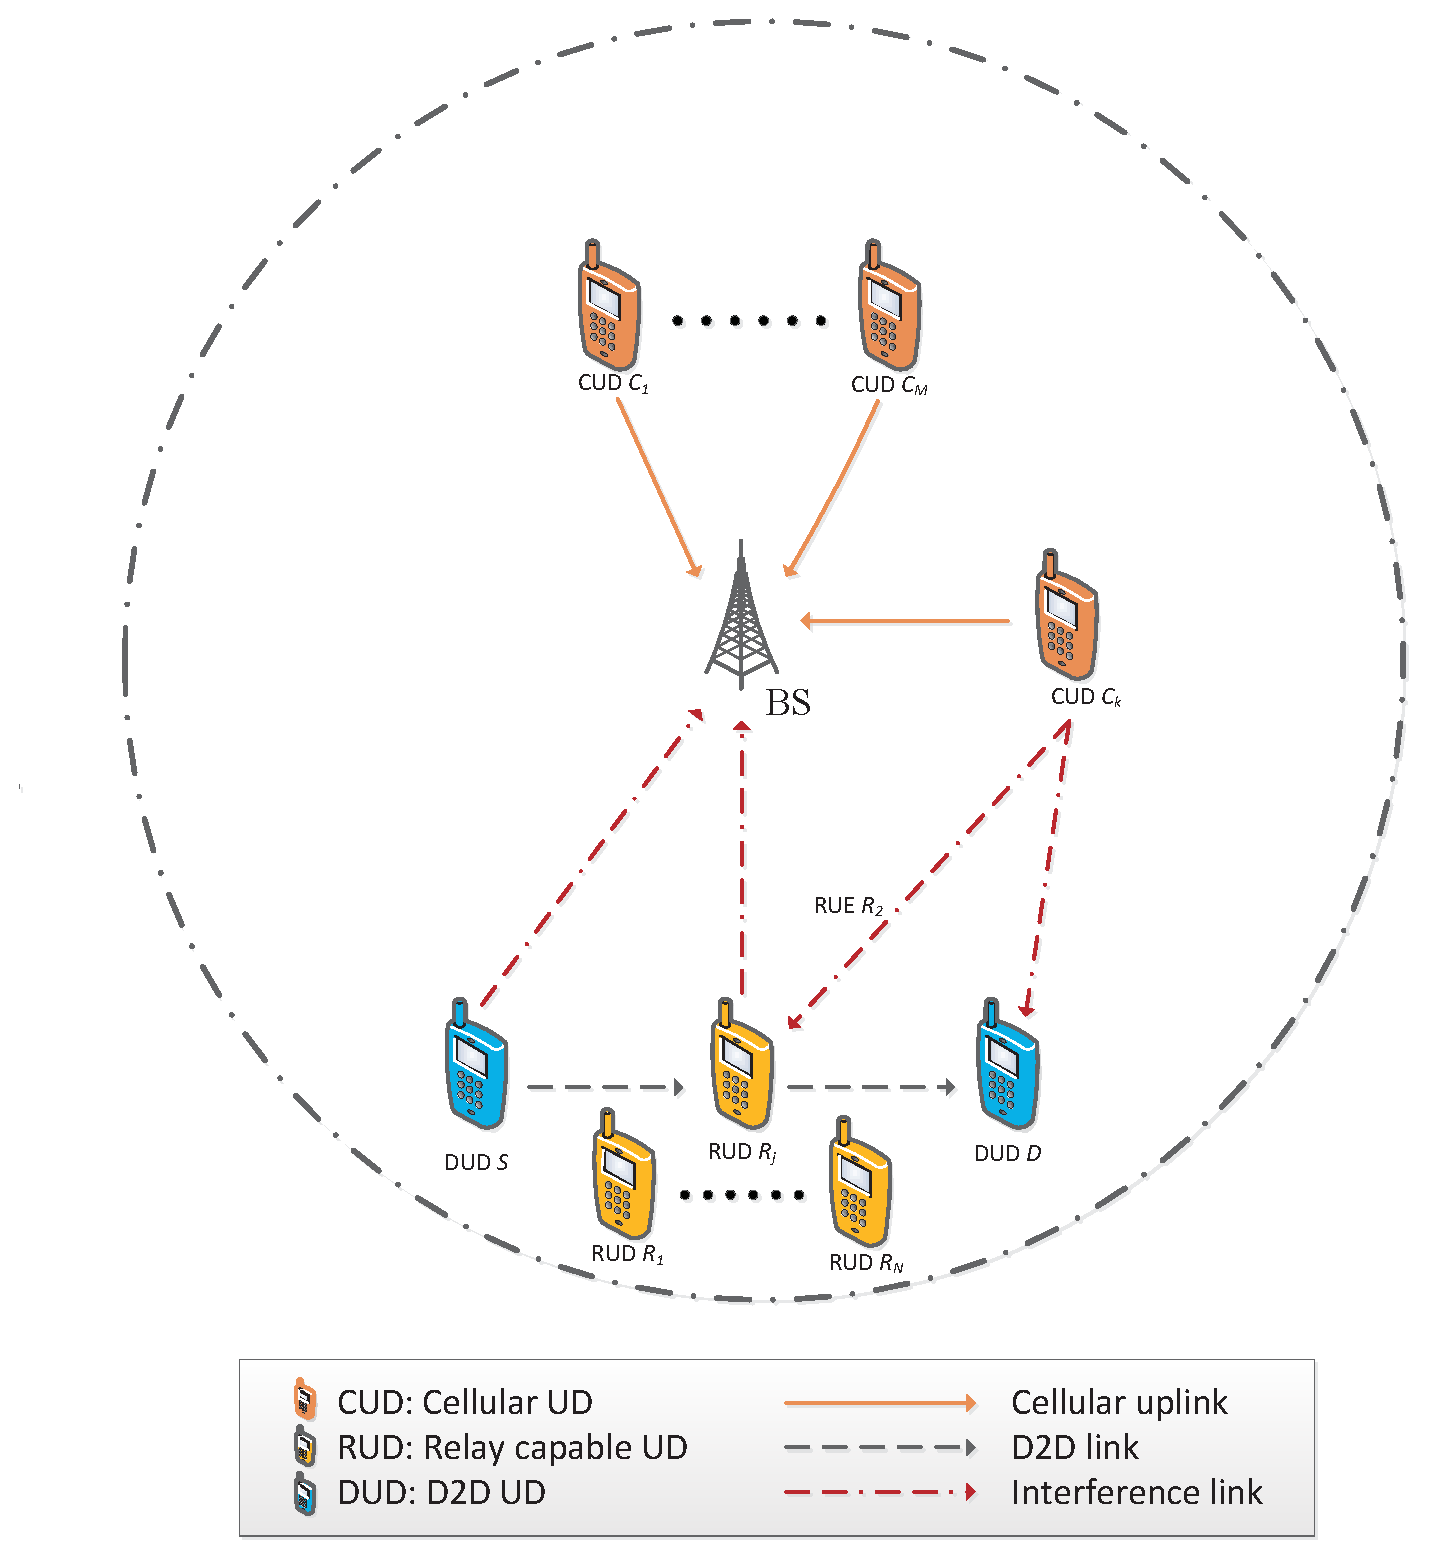
\includegraphics[width=3.5in]{fig1}
%where an .eps filename suffix will be assumed under latex,
% and a .pdf suffix will be assumed for pdflatex; or what has been declared
% via \DeclareGraphicsExtensions.
\caption{The D2D communications scenario underlaying cellular network, where D2D communications reuses the uplink frequency of CUD $C_k$. DUD $S$ denotes the source D2D UD and DUD $D$ denotes the destination D2D UD. RUD $R_j$ is the selected relay UD.}
\label{fig_success}
\end{figure}

Moreover, presume that $M$ CUDs use $M$ separated cell uplink channels which have same bandwidth and can be reused by D2D communications. Depending on these assumptions, we only consider the interference from the reused CUD to the RUD and the $D$ and the interference from the $S$ and RUD to the BS.

In addition, assumed that the BS can acquire the channel state information(CSI) of all links and that the D2D mode, RUD and reuse uplink selection is decided by the BS. Besides, we assume that both CUD uplink channel and D2D link should meet the minimum SINR requirement.

The channel model can be expressed as \cite{6560489}:
\begin{equation}
|{h_{s,d}}|^{2} = K_{0}\beta_{s,d}\zeta_{s,d}\cdot L_{s,d}^{-\alpha}
\end{equation}
$|{h_{s,d}}|^{2}$ is the channel gain between two UDs or between a UD and the BS. $K_{0}$ is a constant determined by cellular parameters. $\beta_{s,d}$ denotes slow fading with log-normally distribution. $\zeta_{s,d}$ denotes fast fading with exponential distribution. $\alpha$ is the path loss exponent and $L_{s,d}$ is the distance between $s$ and $d$

The purpose of this paper is to efficiently utilize cellular frequency resources, RUD residual energy and RUD buffer state to minimize transmission time and maximize total amount of transmission data, before the communications between the source and the destination becomes unavailable. Let $T\left(\chi\right)$ represent the file transmission time of method $\chi$, in other words, the transmission time since the first packet is transmitted by the $S$ until the last packet is received by the $D$, the problem can be expressed as
\begin{align}
&\displaystyle \min _{\mathcal {\chi}} ~T(\mathcal {\chi})
\\[-5pt]&\text {subject to} ~ \sum T_{j} \leq \tau_j(1) , \quad \forall j , \tag{2a}
\\[-1.5pt]&\qquad \qquad ~ j\in\left[1,2,\ldots,N\right] , \tag{2b}
\end{align}
where $\sum T_{j}$ denotes RUD $R_{j}$ total working time, $N$ denotes the total number of packet, and $ \tau_j(1)$ denotes the residual work time of relay $R_j$ in time slot 1.

\section{EABA Relay Selection Method}
As discussed above, an optimal link should be selected by the BS according to transmission rate, RUD residual energy and RUD buffer state. Therefore, we show the methods which establish the transmission rate of the link between DUD and RUD and the residual energy and buffer state of RUD. We will also propose the EABA method for solving the problem in Section \uppercase\expandafter{\romannumeral2}.

\subsection{Link Transmission Rate Estimation}
As shown in Fig. 1, the link transmission rate is derived in this subsection. Let $P_{C_i},P_S$, and $P_{R_j}$ denotes the transmission power of the CUD $C_i$, the $S$, and the RUD $R_j$, respectively. RUD $R_j$ is working in half-duplex mode. If link $S \rightarrow R_j$ is selected as the transmission link and the uplink channel of $C_i$ $(i \in [1,2,\ldots,M])$ is selected as the multiplex channel, the signal received at $R_j$ can be expressed as
\begin{equation}
y^i_{S,R_j} = h_{S,R_j}\cdot x_S + h_{C_i,R_j}\cdot x_{C_i} + n_0
\end{equation}
where $x_S$ is the signal transmitted from the $S$, $h_{C_i,R_j}\cdot x_{C_i}$ denotes the interference from CUD $C_i$ to $R_j$, $n_0$ is additive white Gaussian noise (AWGN), i.e., $n_0 \sim (0,\sigma^2)$. If link $R_j \rightarrow D$ is selected as the transmission link and the uplink channel of $C_k$ $(k \in [1,2,\ldots,M])$ is reused, the signal received at destination DUD $D$ can be expressed as
\begin{equation}
y^k_{R_j,D} = h_{R_j,D}\cdot x_{R_j} + h_{C_k,D}\cdot x_{C_k} + n_0
\end{equation}
where $x_S$ is the signal transmitted from $R_j$, $h_{C_k,D}\cdot x_{C_k}$ denotes the interference from CUD $C_k$ to $D$.

The SINRs of $R_j$ and the $D$ are
\begin{equation}
\gamma^{i}_{S,R_j} = \frac{P_S|{h_{S,R_j}}|^{2}}{P_{C_i}|{h_{C_i,R_j}}|^{2} + \sigma^2} ,\gamma^{k}_{R_j,D} = \frac{P_{R_j}|{h_{R_j,D}}|^{2}}{P_{C_k}|{h_{C_k,D}}|^{2} + \sigma^2}
\end{equation}
respectively. The achievable data rate of link $S \rightarrow R_j$ and $R_j \rightarrow D$ can be expressed as
\begin{equation}
R_{S,R_j} = B\log_2(1 + \gamma^{i}_{S,R_{j}}),R_{R_j,D} = B\log_2(1 + \gamma^{k}_{R_j,D})
\end{equation}
respectively, where $B$ denotes the channel bandwidth.

Likewise, the SINRs of BS are
\begin{equation}
\gamma^{j}_{C_i,B} = \frac{P_{C_i}|{h_{C_i,B}}|^{2}}{P_S|{h_{S,B}}|^{2} + \sigma^2} ,\gamma^{j}_{C_k,B} = \frac{P_{C_k}|{h_{C_k,D}}|^{2}}{P_{R_j}|{h_{R_j,B}}|^{2} + \sigma^2}
\end{equation}
respectively, where B in this equation denotes BS.

\subsection{RUD Residual Energy And Buffer State Estimation}
Owing to the finite energy of the relay, the relay only forwards a finite amount of data before the energy is exhausted. Thus, even though a relay has sufficient buffer size, it's no use sending more data to the relay than it can forward later. To take this into account, we should know the data size can be transmitted by RUD $R_i$ under the residual energy.

Let $E_{1},E_{2},\ldots,E_{j},\ldots,E_{N}$ denotes the total energy of $N$ RUDs, respectively. To describe the influence of the discharge current and transmission power of each RUD on RUD remaining work time, Peukert's Law \cite{6981957} is expressed as
\begin{equation}
\tau_j = E_j/I^{\alpha}_j
\end{equation}
where $\tau_j$ is the remaining work time of $R_j$, $I_j$ is discharge current, and $\alpha$ is the Peukert constant and its usually equal to 1.3 \cite{6981957}. Using $P_{R_j}$ denotes the transmission power of $R_j$, the discharge current can be expressed as
\begin{equation}
I_j = P_{R_j} / V_0
\end{equation}
where $V_0$ denotes the discharge voltage of each UD and predefine the same $V_0$ for each UD.

Therefore, we can establish the remaining work time of each RUD which we know residual energy, transmission power, and discharge voltage. In this paper, the transmission power of each UD is predefined as a fixed value, so we can use the remaining operation time $\tau_j$ denotes the residual energy of RUD $R_j$. Then the minimum data size transmitted by RUD $R_j$ can be expressed as
\begin{equation}
\theta_j = R_{min} \cdot \tau_j
\end{equation}
where $R_{min}$ is the minimum transmission speed of RUD $R_j$

Moreover, the energy of the selected relay is decreased, i.e., $\tau_j(t+1) = \tau_j(t) - tran_j(t)$, where $tran_j(t)$ denotes the transmission time of RUD $R_j$. $Q_j(t)$ is the amount of data stored in RUD $R_j$, so $e_j(t) = L_j -  Q_j(t)$, where $L_j$ denotes the total buffer size of RUD $R_j$, $e_j(t)$ is the RUD $R_j$'s buffer size which can be used at the starting of time slot $t$. And then, the $tran_j(t)$ can be expressed as
\begin{equation}
tran_j(t) = \begin{cases}T & R_{R_j,D}(t)\cdot T \leq Q_j(t)\\Q_j(t)/R_{R_j,D}(t) & R_{R_j,D}(t)\cdot T > Q_j(t)\end{cases}
\end{equation}
where $T$ is duration of a time slot, and $R_{R_j,D}(t)$ is the data rate of link $R_j \rightarrow D$ at time slot $t$.

\subsection{EABA Strategy}
For the purpose of transmitting the file as quickly as possibly, Energy-Aware and Buffer-Assisted (EABA) executes depending on the following theory: the relay which has a lot of residual energy and buffer space should  have a higher priority to recept data. On the other hand, if the relay has a large number of data in its buffer, it should get a higher priority to transmit data to the destination. What's more, a link with a high SINR, which means that more data will be transmitted at a time slot, should have a higher chance to transmit data.

In the EABA method, the BS calculates the weight of every link $S \rightarrow R_j$ as
\begin{equation}
W_{S\rightarrow R_j} = min(\theta_j - Q_j,e_j) \cdot R_{S\rightarrow R_j} \cdot K[\gamma_{S\rightarrow R_j} \geq \gamma_d)]
\end{equation}
while $K[x]$ is zero when x is false and one when x is true. Hence, a link $S \rightarrow R_j$ get a valid weight only when RUD $R_j$ has enough buffer space and residual energy, and the link SINR must no less than the predefined SINR requirement for D2D link.

\begin{algorithm}[!t]
\caption{EABA Relay Selection Method}
\begin{algorithmic} [1]
\STATE {Each RUD calculates the minimum data size that can be transmitted by itself using (10) and sends residual energy and buffer state to the BS.}
\STATE{The BS computes the weight for link $S \rightarrow R_j$ using (12).}
\STATE{The BS computes the weight for link $R_j \rightarrow D$ using (13).}
\STATE {Under BS controls, the best link is selected based on (14).}
\end{algorithmic}
\end{algorithm}

Similarly, for link $R_j \rightarrow D$, the BS calculates the weight as
\begin{equation}
W_{R_j \rightarrow D} = Q_j \cdot R_{R_j \rightarrow D} \cdot K[\gamma_{R_j \rightarrow D} \geq \gamma_d)]
\end{equation}

According to (13), a link $R_j \rightarrow D$ get a valid weight only when relay $R_j$ has data stored in its buffer.

After adopting EABA method calculating the weight, the link $l_{max}$ which has the highest weight is selected, where
\begin{equation}
l_{max} = \arg \max_{l \in \{S \rightarrow R_j\} \cup \{R_j \rightarrow D\}}\{W_l\}
\end{equation}

Algorithm 1 shows the execution process of the EABA method. The EABA method considers transmission rate of each link, residual energy and buffer state of each relay, so the BS needs to know all of there information. When the link with the highest weight is activated by BS, the BS will notify the whole D2D network either the $S$ should transmit to the selected relay or the selected relay  transmit to the $D$.
%Fig2
\begin{figure}[!t]
\center
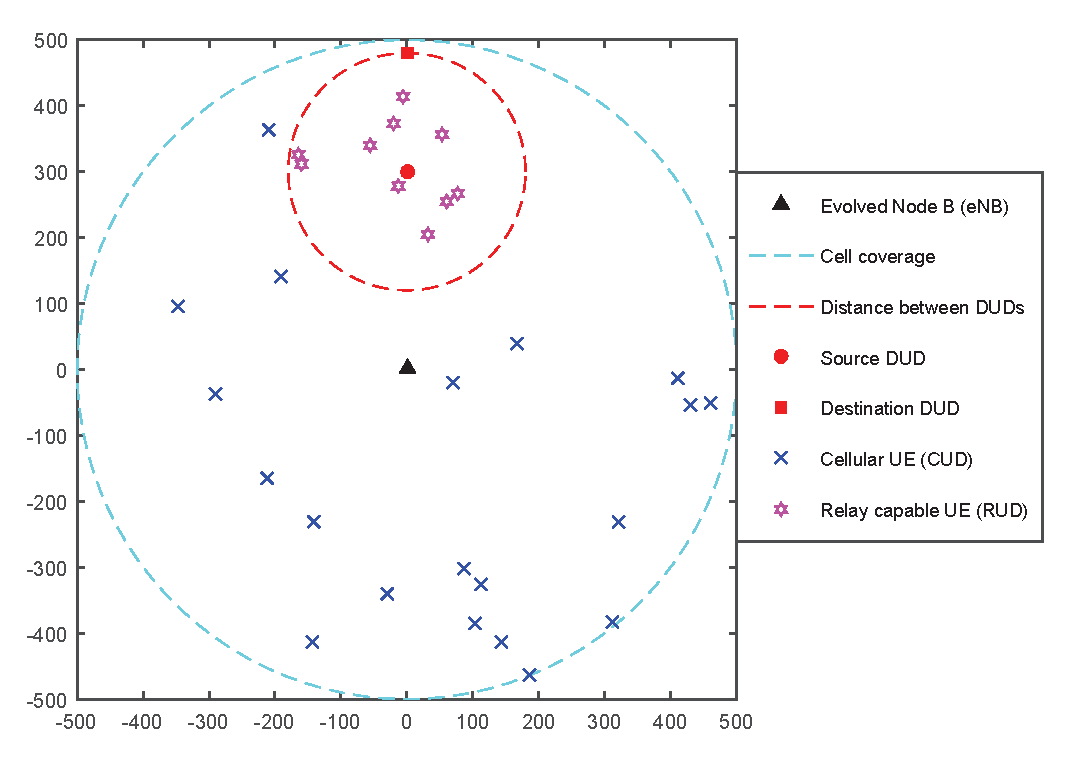
\includegraphics[width=3.5in]{fig2}
%where an .eps filename suffix will be assumed under latex,
% and a .pdf suffix will be assumed for pdflatex; or what has been declared
% via \DeclareGraphicsExtensions.
\caption{The simulation of the scenario. The distance between the $S$ and $D$ is 220m.}
\label{fig_scenario}
\end{figure}

As long as the network is available, the procedure of EABA continues. Depending on the above discussion of the EABA method, if relay $R_j$ has data stored in its buffer, $R_j$ will have enough energy to transmit that data. Note that there will be a time slot in which that link $R_j \rightarrow D$ will have a good channel condition, $R_j$ will transmit the data which has been stored in $R_j$ to the $D$ successfully. Hence, if the network becomes unavailable, there will be no data stored in relay $R_j$.

\section{Simulation Results}
In this section, we provide simulations in MATLAB to evaluate the proposed relay selection method. Simulation is performed in a single cellular, and we assume that the cellular radius is 500 meters. We also assume that all CUDs are random distributed in the cellular. Besides, there are only two DUDs (the $S$ and the $D$), and all RUDs are random distributed in  a circular area with the distance between the $S$ and the $D$ as its radius and the $S$ as its center. The scenario of the simulation is shown in Fig. 2, and Table \uppercase\expandafter{\romannumeral1} lists main parameters used in this paper. Since all UDs were re-deployed random in different test, we did 100,000 times experiments at the same scenario for getting an average result.

The EABA relay selection method is validated by the simulations as shown in Fig. 3, 4. To evaluate the necessity of it, we make a comparison of "EABA relay selection" with "random relay selection" and "rate based relay selection". All the three relay selection methods assume that direct D2D mode is unavailable, that is to say, the three methods are only working in relay-aided D2D mode. Moreover, we also ignore the time and energy consumption caused by calculation. The "random relay selection" selects a link randomly; The "rate based relay selection" selects a link with maximum SINR, i.e., the maximum transmission rate; while the "EABA relay selection" selects the link which is calculated by the formula proposed in Section \uppercase\expandafter{\romannumeral3}.
%Table 1
\begin{table}[!t]
  \centering
  \scriptsize
  \caption{Simulation parameters}
  \label{tab:notations}
  \begin{tabular}{m{3cm}m{3cm}}
    \\[-2mm]
    \hline\\[-2mm]
    {\bf  Parameters}& {\bf Value}\\
    \hline
    \hline
    \vspace{1mm}\\[-3mm]
    Cellular radius      &    500 m\\
    \hline
    \vspace{1mm}\\[-3mm]
    Noise density &    -174 dBm/Hz \\
    \hline
    \vspace{1mm}\\[-3mm]
    UE transmit power  &  24 dBm\\
    \hline
    \vspace{1mm}\\[-3mm]
    The number of CUD  &  20 \\
    \hline
    \vspace{1mm}\\[-3mm]
    The number of DUD  &  10 \\
    \hline
    \vspace{1mm}\\[-3mm]
    Path-loss exponent ($\alpha$) &  4 \\
    \hline
    \vspace{1mm}\\[-3mm]
    Path-loss constant ($K_0$) &   0.01\\
    \hline
    \vspace{1mm}\\[-3mm]
    SINR requirements ($\gamma_c,\gamma_d$) &  20 dB \\
    \hline
    \vspace{1mm}\\[-3mm]
    Slow fading ($\beta_{s,d}$) &  Log-normal distribution with mean value of zero and standard deviation of 10\\
    \hline
    \vspace{1mm}\\[-3mm]
    Fast fading ($\zeta_{s,d}$) &  Exponential distribution with mean value of one\\
    \hline
    \vspace{1mm}\\[-3mm]
    Packet number &  50 \\
    \hline
    \vspace{1mm}\\[-3mm]
    Packet size &  1024 bits\\
    \hline
    \vspace{1mm}\\[-3mm]
    A unit time slot ($\triangle T$) &  $1 \mu s$\\
    \hline
    \vspace{1mm}\\[-3mm]
    RUD total energy ($E_i$) &  Randomly distributed in [0,1440] mAh \\
    \hline
  \end{tabular}
\end{table}
%Fig3
\begin{figure}[!t]
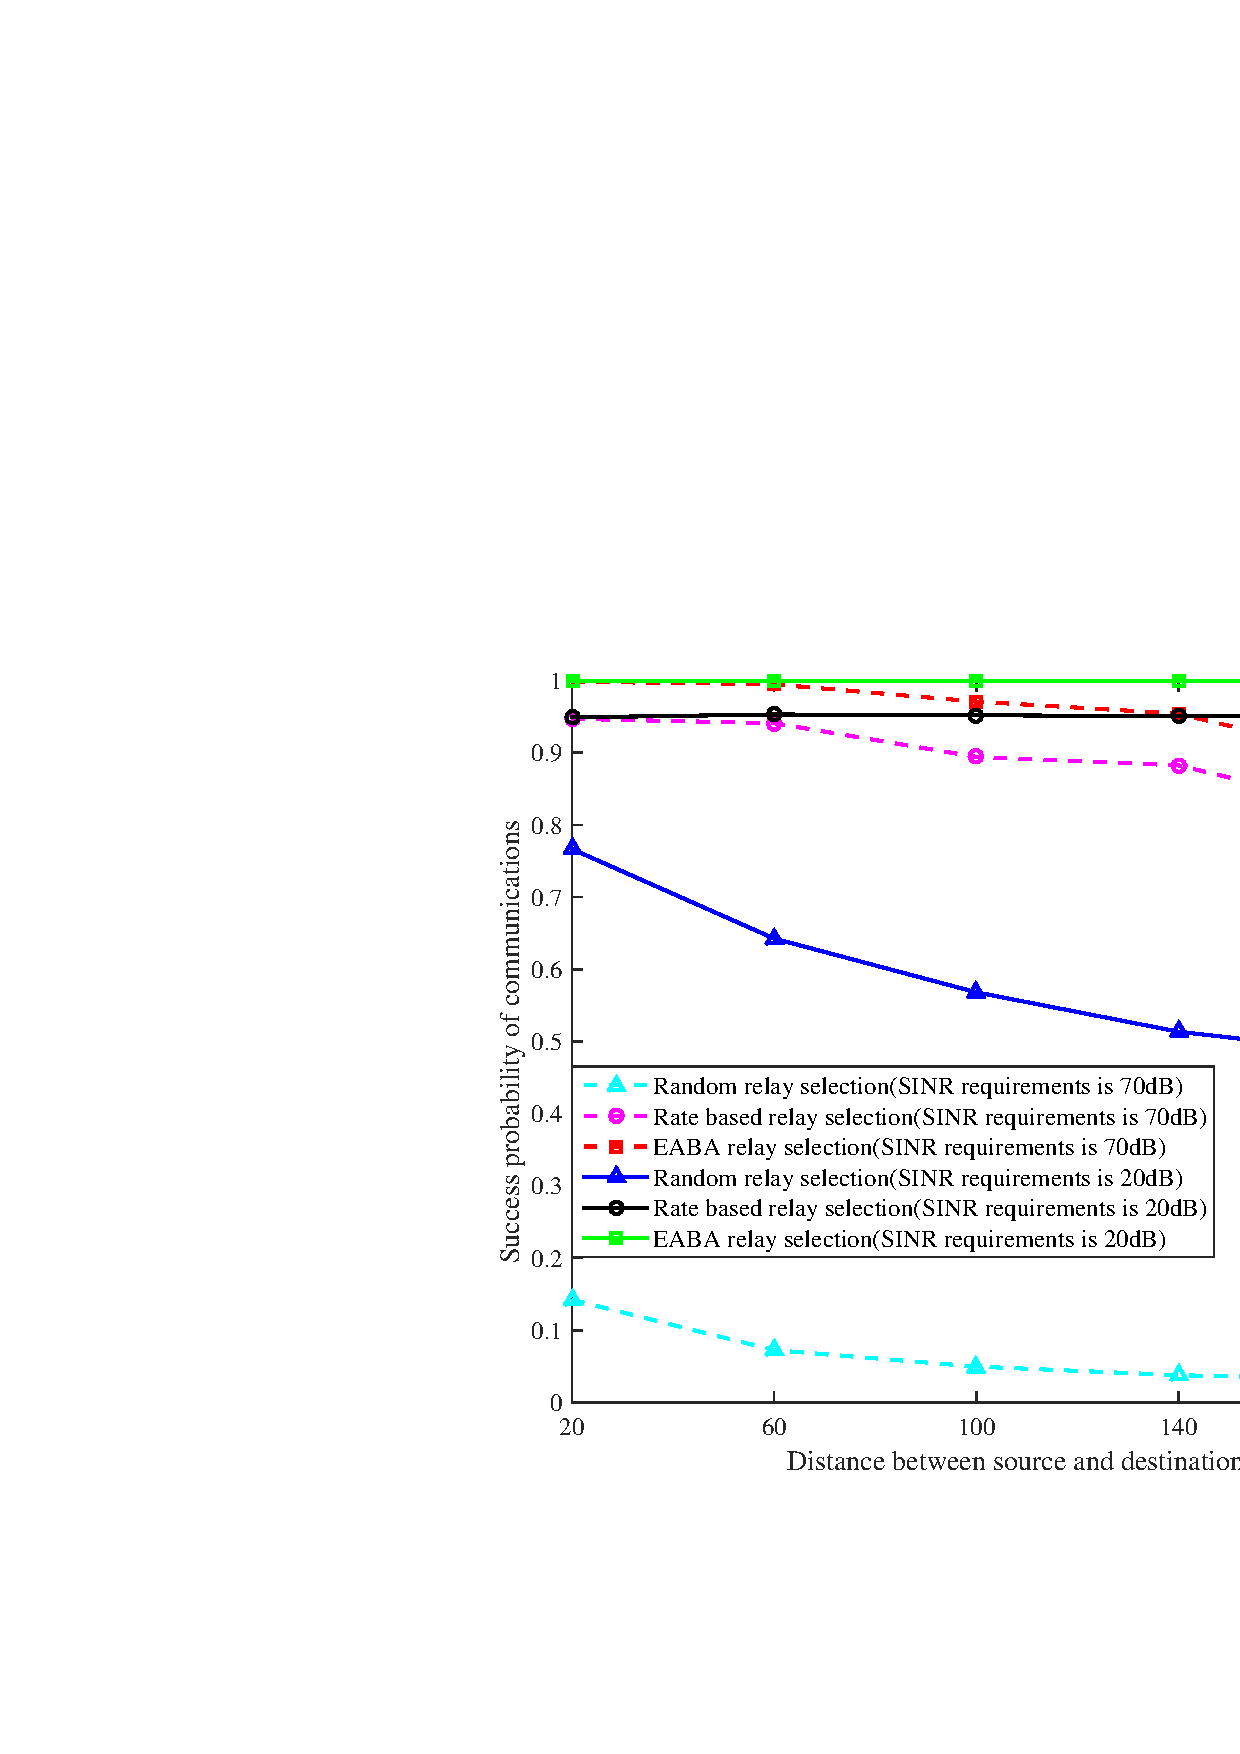
\includegraphics[width=3.5in]{fig3.pdf}
%where an .eps filename suffix will be assumed under latex,
% and a .pdf suffix will be assumed for pdflatex; or what has been declared
% via \DeclareGraphicsExtensions.
\caption{The probability of successful communications using the three relay selection methods. The RUD buffer size is 5, the uplink channel bandwidth is 720 kHz.}
\label{fig_success}
\end{figure}

%Fig4
\begin{figure}[!t]
\center
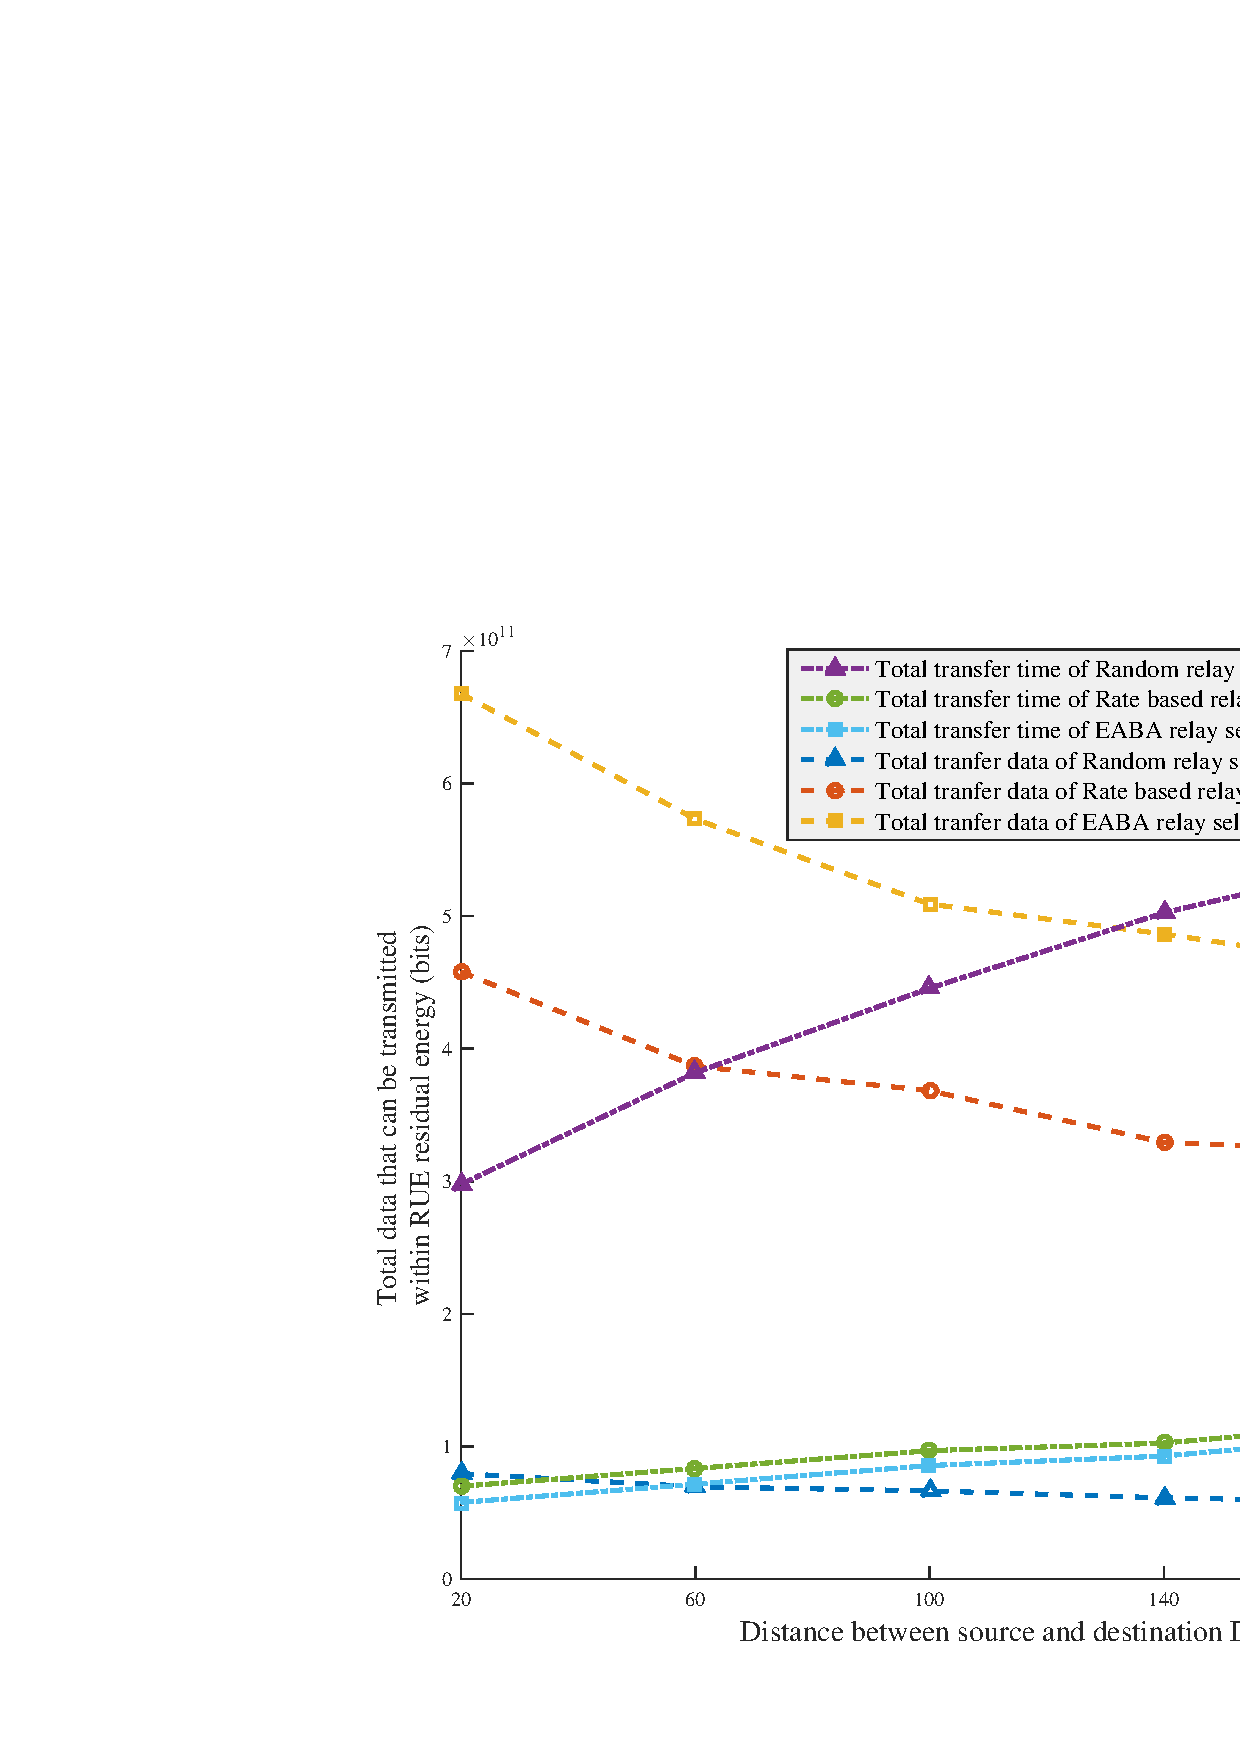
\includegraphics[width=3.5in]{fig4.pdf}
%where an .eps filename suffix will be assumed under latex,
% and a .pdf suffix will be assumed for pdflatex; or what has been declared
% via \DeclareGraphicsExtensions.
\caption{The total transmission time and the total amount of data transmitted with three relay selection methods. The RUD buffer size is 5, the uplink channel bandwidth is 720 kHz.}
\label{fig_time}
\end{figure}

Fig. 3 demonstrates the probability of successful communications using the three relay selection methods. As the distance between DUDs $S$ and $D$ decreases, the chances of successful communication are greatly improved. The result is very plausible, the channel gain of link between DUDs and RUDs will increase with an decreasing distance, which will improve the chance of successful communication. Specifically, the EABA method presents the best performance. The reason is that random relay selection method randomly selects a link, SINR of which may not meet the requirement and subsequently lead to communication failure. Even though the rate based relay selection method selects a link from $S$ to RUD with maximum link transmission rate, but the RUD does not have enough buffer space or residual energy which may lead to communication failure. Furthermore, no matter which method is applied, D2D communication achieves higher success probability under a lower link SINR requirement.

Fig. 4 shows that the total data transmission time decreases when the distance between $S$ and $D$ is expanded. The transmission rate of both $S$-to-RUD and RUD-to-$D$ links will be reduced by expanding separation distance, directly resulting in a decreased amount of transmission data in all of links. Thus, the total transmission time will go up. In the three methods, the EABA method has the minimum total transmission time, because it has a higher data rate and the probability of successful communications. The random relay selection method shows the worst performance, due to its lowest data rate of link and lower probability of successful communications. Although rate based relay selection method select the fastest link, but the lower success probability of communications leading to a lower transmission time than EABA method.

Fig. 4 shows that the influences of the distance between the $S$ and $D$ on the total amount of data. As the distances increasing, the path loss will significantly enhance, leading to a decreasing link transmission rate. Moreover, under the same cellular parameters, the random method affords a much worse performance than the other two selection methods, because both the data rate of selected link and residual energy of RUD are neglected. Despite rate based method chooses the link which has highest transmission rate to transmit data, it will consume all of the energy of the system quickly, because it is not consider the residual energy of RUD. The EABA method provides the best performance, because it not only ensure the system work more time, but also ensure the link data rate.

\section{Conclusion}
In this paper, we designed an Energy-Aware and Buffer-Assisted (EABA) relay selection method that jointly considered transmission rate, RUD residual energy, and RUD buffer state. We also described the computational processes of the transmission rate, RUD residual energy, and RUD buffer state. Specially, we established a relay selection method which selected the best link instead of selecting best relay. Simulation results showed that the proposed method provided the better overall transmission performance compared with other relay selection methods.

\section*{Acknowledgment}
This work was supported by the National Key Technology R\&D Program (No.2015BAI01B14) and the Fundamental Research Funds for the Central Universities.
% references section
% trigger a \newpage just before the given reference
% number - used to balance the columns on the last page
% adjust value as needed - may need to be readjusted if
% the document is modified later
\bibliographystyle{IEEEtran}
\bibliography{ref}

\end{document} 